\documentclass[12pt]{article}
\setlength\parindent{0pt}
\usepackage{fullpage}
\usepackage{amsmath}
\usepackage[margin=0.75in]{geometry}
\usepackage{graphicx}
\setlength{\parskip}{4mm}
\def\LL{\left\langle}   % left angle bracket
\def\RR{\right\rangle}  % right angle bracket
\def\LP{\left(}         % left parenthesis
\def\RP{\right)}        % right parenthesis
\def\LB{\left\{}        % left curly bracket
\def\RB{\right\}}       % right curly bracket
\def\PAR#1#2{ {{\partial #1}\over{\partial #2}} }
\def\PARTWO#1#2{ {{\partial^2 #1}\over{\partial #2}^2} }
\def\PARTWOMIX#1#2#3{ {{\partial^2 #1}\over{\partial #2 \partial #3}} }
\newcommand{\BE}{\begin{displaymath}}
\newcommand{\EE}{\end{displaymath}}
\newcommand{\BNE}{\begin{equation}}
\newcommand{\ENE}{\end{equation}}
\newcommand{\BEA}{\begin{eqnarray}}
\newcommand{\EEA}{\nonumber\end{eqnarray}}
\newcommand{\EL}{\nonumber\\}
\newcommand{\la}[1]{\label{#1}}
\newcommand{\ie}{{\em i.e.\ }}
\newcommand{\eg}{{\em e.\,g.\ }}
\newcommand{\cf}{cf.\ }
\newcommand{\etc}{etc.\ }
\newcommand{\Tr}{{\rm tr}}
\newcommand{\etal}{{\it et al.}}
\newcommand{\OL}[1]{\overline{#1}\ } % overline
\newcommand{\OLL}[1]{\overline{\overline{#1}}\ } % double overline
\newcommand{\OON}{\frac{1}{N}} % "one over N"
\newcommand{\OOX}[1]{\frac{1}{#1}} % "one over X"



\begin{document}
\Large
\centerline{\sc{Homework 7}}
\normalsize
\centerline{\sc{Due Monday, 8 April}}
\centerline{Submit to your TA's mailbox before the Physics Building closes}

\begin{enumerate}

\item{An ambitious kestrel of mass 100 grams sees a tasty pigeon flying below it and dives to catch its dinner. The pigeon has a mass of 200 grams. It is flying horizontally at
10 m/s when the kestrel, diving straight down, grabs it.

After the kestrel catches the pigeon, the two of them are moving in a direction 45 degrees below the horizontal. How fast was the kestrel moving before it caught the pigeon?}

\item{In forensic science, it is useful to measure the speed at which firearms propel bullets. Before modern instruments, this was done with a device called a ``ballistic pendulum'', consisting of a block of some soft material hanging from the end of a string.
The experimenter fires a bullet into the block, which lodges into it; the block swings up at an angle. By measuring the angle, the experimenter can determine the velocity of the bullet.

Suppose that you are a detective trying to measure the velocity of the bullets fired from a particular gun. You construct a ballistic pendulum out of a string of length 50 cm and a clay block of mass 2 kg, and fire a bullet into it. If the bullet has
a mass of 2.6 grams and the pendulum swings up to an angle 13.4 degrees, how fast was the bullet traveling when it struck the block?}

\item{In the classic computer game {\it Portal}, the player is asked to solve
puzzles with the use of a ``portal device'', which can create two connected portals
on, for example, the floor and a wall. An object entering one portal with speed $v$
will exit the other with the same speed. Here's an illustration:

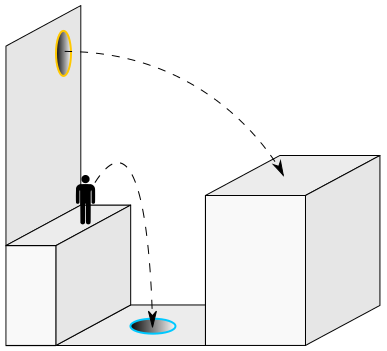
\includegraphics[width=0.4\textwidth]{Portal_physics-2.png}

The game's narrator helpfully explains that ``Forward momentum, a product of mass
and velocity, is conserved between portals. In layman's terms: {\bf speedy thing
goes in; speedy thing comes out.}''

\begin{enumerate}
\item{Is this an accurate statement of the law of conservation of momentum? As the
narrator claims, does such a device conserve momentum? If not, why not?}
\item{Does this device conserve kinetic energy?}
\item{Does it conserve total energy (that is, kinetic energy $\frac{1}{2}mv^2$
plus gravitational potential energy $mgy$?}
\end{enumerate}
}

\item{When an extremely massive star reaches the end of its life, the core of the star is no longer able to support its own weight, and it collapses into a very dense ball of neutrons. This precipitates the star to explode in a supernova.

Suppose that the core of a dying star has a diameter of 50000 km and rotates slowly, spinning once per day. After the supernova, it collapses into a neutron star of diameter 50 km. 

\begin{enumerate}
\item How quickly will the neutron star be spinning?
\item In $g$'s, what is the centripetal acceleration at the surface of this neutron star?
\end{enumerate}
}
\item Consider the demo that you saw in class, in which a person stands on a platform that is free to rotate. They are initially at rest.

Someone hands them a bicycle wheel of 
radius $r=30$ cm that is full of concrete, and thus has a mass of $m=4$ kg\footnote{Remember that the moment of inertia of any object where all of the mass is 
the same distance from the center is $I=mr^2$.} You may model the person as a cylinder ($I=\frac{1}{2}mr^2$) of mass 80 kg and radius 20 cm. 

Suppose that the bike wheel is initially spinning horizontally at an angular velocity of $\omega_0 = 50$ rad/s. The person turns the bike wheel over, so that it is
spinning in the opposite direction at the same angular velocity.

What will happen to the angular velocity of the person after they do this?

\item Commercially-available hybrid vehicles, such as the Toyota Prius, use electrical batteries to store energy for later use. However, Formula One racecars have used
a flywheel to store energy. When the car applies its brakes, translational kinetic energy of the car is converted to rotational kinetic energy of a large wheel;
later, when the driver wants extra power, the wheel can be coupled to the drivetrain of the car, using that kinetic energy to supplement the power from the engine.

The ``Flybrid'' hybrid system uses a 5 kg wheel with a radius of 12 cm. When this system is engaged, it can provide an extra 60 kW of power to the car for 7 seconds.

\begin{enumerate}
\item How much energy does this system store?
\item At what angular velocity must the wheel spin to store this much energy? Convert your answer to revolutions per minute. Does this result surprise you?
\item What is the centripetal acceleration of a point on the edge of this wheel? Can you think of any engineering or safety challenges in building these systems?
\end{enumerate}

\end{enumerate}

\end{document}
